\documentclass[Rapport/Rapport_main.tex]{subfiles}
\begin{document}
\section{Software test}
I det følgende afsnit beskrives hvordan CarnGo testes, herunder hvilke redskaber, frameworks og principper, som er anvendt i praksis. For at sikre, at applikation opfører sig som forventet og opfylder kravene, er det essentielt at teste softwaren grundigt. Software test skal i denne sammenhæng forstås som, at man systematisk og objektivt verficerer en software enheds tilstand og opførsel baseret på nogle objektive og prædefinerede kriterier eller krav. Med systematisk og objektivt menes der, at testen skal være målbar, og at det skal være muligt for en anden at gentage testen med identiske resultater. At kriterierne er objektive betyder, at der ikke er plads til fortolkning af resultatet. For flere informationer vedrørende applikationens software tests henvises til bilaget \textbf{X}.

\subsection{Unit Testing}
En unit test er et automatiseret stykke kode, som kalder den enhed, der skal testes. Den grundlæggende idé er at påvirke enheden for herefter at tjekke nogle antagelser omkring slutresultatet. Unit tests anvendes i vidt omfang til at teste applikationen CarnGo - hver enkelt test case er struktureret på samme vis og består af tre trin:
\begin{itemize}
    \item \textit{Arrange} objekter, opret og opsæt dem efter behov
    \item \textit{Act} på et objekt, udfør aktiviteten som skal testes
    \item \textit{Assert} at resultatet er som forventet
\end{itemize}
Til at skrive testene er der anvendt frameworks kaldet NUnit og NSubstitute, som beskrevet i forgående afsnit. Dette gør test cases lettere at skrive og vedligeholde, og de kan hurtigt eksekveres ved tryk på en knap.

\subsection{Continuous Integration}
For at undgå problemer med integration af softwaren er der i projektet anvendt en praksis kaldet Continous Integration. Det indebærer at teamets medlemmer integrerer ofte, og at hver integration verificeres af et automatisk build. Github er anvendt som remote repository, og Jenkins er anvendt som build server. Det er konfigureret på en sådan vis, at Jenkins bliver triggered, når der pushes til Git serveren. Dermed startes et build job, hvor projektet bygges og test køres, og først herefter kan der igen pulles fra serveren. Denne fremgangsmåde sikrer, at integrationsfejl opdages og korrigeres tidligt i processen. Samtidig er man aldrig langt fra et fungerende build, og som udvikler får man løbende feedback i forhold til kodens og testens kvalitet.

\subsection{Coverage}
For at sikre kvaliteten af testene der løbende er blevet set på, hvor meget af applikationens kode, der er dækket af tests. Dette betegnes Test Coverage, og det giver et billede af, hvilke områder af programmet, der bliver anvendt eller aktiveret i applikationens test suite. Coverage giver et kvantitativt mål for, hvor godt testene dækker koden, og denne viden kan anvendes til systematisk at udvide eller tilføje test cases indtil alt applikationskoden er omfattet. Der skelnes mellem forskellige former for Coverage og der er ulemper forbundet med dem alle. Generelt er fuld coverage heller ikke ensbetydende med ingen fejl, men det anvendes alligevel i projektet, da det er et simpelt og objektivt mål for kvaliteten af tests. Til at beregne Coverage for CarnGo er der anvendt værktøjet dotCover, og der sigtes efter 100\% Coverage. Den er dog endt med at være væsentligt lavere, med blot \textbf{X}\%, hvilket kan tilskrives...

\subsection{Boundary Value Analysis \& Equivalence Partitions}
Det vil oftest ikke være realistisk at lave udtømmende tests for alle sæt af test data, og særligt ikke hvis der er mange mulige input kombinationer. Boundary Value Analysis (BVA) har til formål at identificere de input værdier, hvor output ændrer værdi eller validitet. Ved at teste på begge sider af disse grænseværdier kan man reducere antallet af test cases, så man arbejder med et sæt af \textit{tilstrækkelige} og \textit{nøvendige} test cases frem for et udtømmende sæt. BVA anvendes altid i kombination med Equivalence Partitions (EP). En EP er en del af alle mulige inputs, som resulterer i samme output eller den samme form for opførsel. Når EPs er identificeret testes med mindst én værdi fra hver EP og ikke samtlige værdier. Tilsammen hjælper BVA og EPs med at sikre, at man udtænker de rigtige test cases og ikke tester for meget, og de er således et godt supplement til Coverage.

\subsection{ZOMBIE}
\textbf{ZOMBIE} er et akronym, der har fungeret som en guide for, hvad der skulle testes i projektet, og de overvejelser der er gjort undervejs. \textbf{Z} står for Zero og indikerer, at de første test scenarier bør være simple post-konditioner for nyligt oprettede elementer. F.eks. kan det testes, at en tom collection indeholder nul elementer, eller at der er nul kald af et nyoprettet objekt. \textbf{O} står for One, som er den næste case, der bør testes. Når man går fra nul til ét input/output/action er der en række nye scenarier, der bør afprøves. Herefter generaliseres scenariet, og der testes nu et Many scenarie (\textbf{M}) med mange inputs/outputs/actions. På denne vis bevæger man sig altid fra simple til mere komplekse testscenarier. \textbf{BIE}-delen af ordet står derimod for de overvejelser, man bør gøre sig undervejs, mens man sigter efter simplicitet i test scenarierne. \textbf{B} står for Boundaries og indikerer, at man bør teste grænseværdier og gøre brug af førnævnte BVA og EPs. \textbf{I} står for Interfaces, da man bør teste alle metoder, events, kaldte interfaces og afhængigheder. Endelig står \textbf{E} for Exceptional Behaviour, da man bør tage højde for og teste uforventet opførsel, timeouts og fejlhåndtering.

\section{Integrationstest}
\subsection{Dependency Tree}
Der er udarbejdet et Dependency Tree for applikationen, hvilket kan ses i figur \ref{fig:dependency_tree}. Det illustrerer afhængighederne mellem klasserne og udgør grundlaget for en integrationstest. Dels kan det bruges til at bestemme, hvilke dele af systemet, der skal integrationstestes, men det er også ofte afhængighederne der dikterer testenes rækkefølge. Det fremgår af figur \ref{fig:dependency_tree} at f.eks. View er afhængig af ValueConverters, og derfor er det relevant at integrationsteste disse to moduler. Omvendt bør Properties ikke testes med ValueConverters, da der ikke er nogen afhængighed mellem disse klasser. 
\begin{figure}[H]
    \centering
    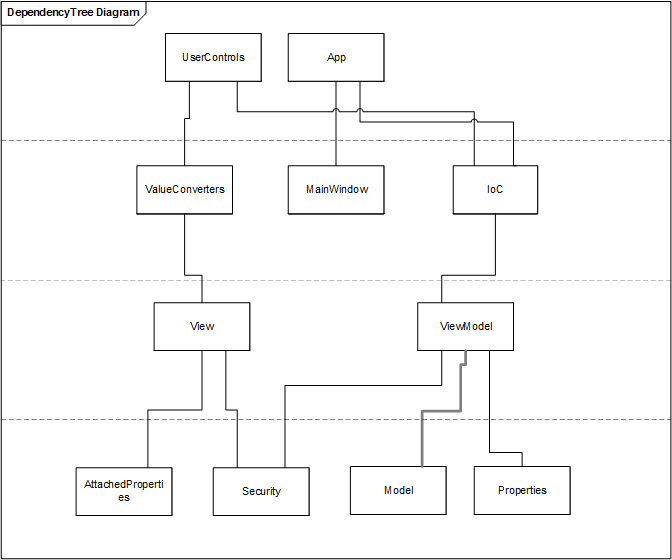
\includegraphics[width=\textwidth]{Rapport/Tests/DepedencyDiagramV2.png}
    \caption{Dependency Tree for CarnGo}
    \label{fig:dependency_tree}
\end{figure}

\subsection{Integrationsplan}

\end{document}